\section{Fase B: integración Monte Carlo y remuestreo}

\subsection{Estimadores como integrales Monte Carlo}

Las cantidades de interés son momentos de $\pi_\beta$ y se estiman con promedios sobre la cadena. Con $E_t$ la energía y $m_t=\lVert\sum_i\mathbf S_i\rVert/N$ la magnetización en el barrido $t$,
\begin{equation}
c(T)=\frac{\operatorname{Var}_{\pi_\beta}(\mathcal H)}{N\,k_BT^2},\qquad
\chi(T)=\frac{N\operatorname{Var}_{\pi_\beta}(m)}{k_BT},\qquad
T^*=\arg\max_{T\in[6,20]}c(T).
\label{eq:observables}
\end{equation}
El calor específico $c$ es una varianza escalada: mide cuánto fluctúa la energía y es máximo donde el sistema cambia de régimen. En un sistema finito el máximo queda redondeado. Su posición $T^*$ identifica una temperatura característica o pseudocrítica; la existencia de una singularidad y su tipo exigirían un análisis de tamaño finito. Con campo externo, un máximo no establece por sí solo una temperatura de Curie. Este $T^*$ es el argumento del máximo de una curva estimada, un estadístico no suave, y por eso su incertidumbre se obtiene por remuestreo y no por el método delta. Para ubicarlo entre las temperaturas simuladas se usó el repesado de histogramas de \citet{ferrenberg1988}, $\langle A\rangle_\beta=\sum_tA_tw_t/\sum_tw_t$ con $w_t=e^{-(\beta-\beta_0)\mathcal H_t}$, sobre una rejilla de 0.01~K y con control del tamaño efectivo de Kish de los pesos.

\subsection{Error con datos dependientes: autocorrelación y jackknife por bloques}

Los barridos consecutivos de una cadena están correlacionados. Si $\rho(k)$ es la autocorrelación de la serie, la varianza de su media es aproximadamente $\sigma^2\,\tauint/n$, con
\begin{equation}
\tauint=1+2\sum_{k=1}^{W}\rho(k),\qquad n_{\mathrm{ef}}=\frac{n}{\tauint},
\end{equation}
donde la ventana $W$ es el menor valor con $W\ge6\,\tauint(W)$ \citep{sokal1997,wolff2004}. Esta convención es el doble de la de Sokal, $\tau_S=\tfrac12+\sum_k\rho(k)$, y se usa en el análisis de barridos. El programa oficial de errores trabaja con $\tau_S$ por copia y ventana $W\ge10\tau_S$; el análisis de barridos agrupa autocovarianzas entre copias y usa $W\ge6\tauint$. La diferencia de agregación y ventana impide convertir sus máximos mediante un factor dos exacto. Tratar la serie como independiente subestima el error estándar en un factor $\sqrt{\tauint}$. El tiempo $\tauint$ también se lee como el número de barridos que la cadena necesita para producir una observación nueva, y por eso es la medida natural del costo en pasos Monte Carlo.

Para la varianza dentro de una copia se usó el jackknife por bloques. La serie de $n=10\,000$ barridos se parte en $g$ bloques contiguos de largo $b=n/g$, el estimador se recalcula sin cada bloque y $\widehat{\mathrm{se}}_{JK}=\big[\tfrac{g-1}{g}\sum_j(\hat\vartheta_{(j)}-\bar\vartheta_{(\cdot)})^2\big]^{1/2}$. Se eliminan bloques y no observaciones para conservar la dependencia temporal dentro de cada bloque. El tamaño se eligió a partir de la autocorrelación: en cada temperatura se toma la mediana, sobre las copias, del mayor $\tauint$ entre $E$, $m$, $E^2$ y $m^2$, y $b$ es el menor valor de una lista fija (de 1 a 500 barridos) con $b\ge5\,\tauint$, equivalente a $b\ge10\,\tau_S$. Esa longitud busca reducir la dependencia entre bloques; no proporciona una cota universal del 10~\% para el sesgo de cualquier estimador o función de autocorrelación. Además se exigen $g\ge20$ bloques, con lo que el error relativo del propio error estándar queda cerca de $1/\sqrt{2(g-1)}\approx16~\%$. Las dos condiciones requieren aproximadamente $\tauint\le100$ para la estimación por copia que selecciona el bloque. Los máximos del análisis de barridos, 57 para energía y 946 para magnetización, proceden de otra agregación y ventana y no sustituyen esa regla por temperatura. La tabla oficial conserva el resultado operativo del jackknife: el estado 5 lo satisface en toda la escalera.

\subsection{Bootstrap entre copias}

Las 100 copias de un estado son independientes por construcción, de modo que la copia completa es la unidad de remuestreo. En cada una de $B=50\,000$ réplicas se sortean 100 copias con reemplazo (índice $I=\lfloor100\,U\rfloor$, transformada inversa discreta), se usan las mismas multiplicidades en toda la escalera para conservar la continuidad del camino, se recalcula la curva repesada $c(T)$ y se toma su máximo. Se reportan los intervalos percentil, $[q_{0.025},q_{0.975}]$, y BCa, con corrección por sesgo $z_0$ y aceleración $a$ estimada con el jackknife que deja fuera una copia a la vez \citep{efron1993}. El bootstrap mide la variabilidad entre caminos; no corrige un sesgo común a todos ellos, que solo los diagnósticos de la sección~\ref{sec:convergencia} pueden detectar.

\subsection{Resultado: la temperatura de transición}

\begin{figure}[H]
\centering
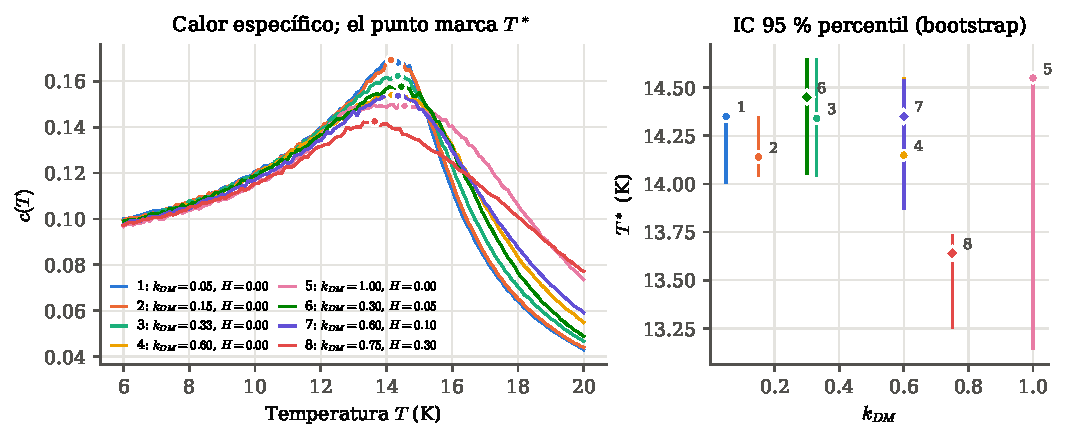
\includegraphics[width=\textwidth]{calor_especifico.pdf}
\caption{Izquierda: calor específico $c(T)$ de los ocho estados, promedio sobre 100 copias; el punto marca $T^*$. Derecha: $T^*$ frente a $\kdm$ con su intervalo percentil del 95~\%; círculos, $\Hex=0$; rombos, $\Hex>0$.}
\label{fig:calor}
\end{figure}

\begin{table}[H]
\centering\small
\caption{Temperatura del máximo de $c$. Bootstrap entre copias con $B=50\,000$. La meseta es el intervalo contiguo de la rejilla fina donde $c\ge c(T^*)-\widehat{\mathrm{se}}$, con $\widehat{\mathrm{se}}$ el error bootstrap de la altura del pico.}
\label{tab:tstar}
\begin{tabular}{ccccccc}
\toprule
Estado & $T^*$ (K) & se (K) & IC 95~\% percentil & IC 95~\% BCa & Meseta (K) & $c(T^*)$\\
\midrule
1 & 14.35 & 0.117 & [14.00, 14.37] & [14.14, 14.45] & [14.35, 14.40] & 0.170\\
2 & 14.14 & 0.068 & [14.04, 14.35] & [13.95, 14.14] & [14.11, 14.14] & 0.170\\
3 & 14.34 & 0.164 & [14.04, 14.65] & [13.85, 14.55] & [14.25, 14.34] & 0.163\\
4 & 14.15 & 0.127 & [14.04, 14.55] & [13.64, 14.15] & [14.15, 14.24] & 0.155\\
5 & 14.55 & 0.445 & [13.14, 14.55] & [13.55, 14.65] & [14.55, 14.58] & 0.151\\
6 & 14.45 & 0.166 & [14.05, 14.65] & [14.05, 14.65] & [14.45, 14.49] & 0.158\\
7 & 14.35 & 0.201 & [13.87, 14.54] & [13.94, 14.55] & [14.35, 14.44] & 0.155\\
8 & 13.64 & 0.127 & [13.25, 13.74] & [13.14, 13.64] & [13.60, 13.64] & 0.143\\
\bottomrule
\end{tabular}
\end{table}

En los ocho estados, $c(T)$ tiene un máximo ancho cerca de 14.3~K (figura~\ref{fig:calor} y tabla~\ref{tab:tstar}). Como verificación independiente, el argumento del máximo recalculado directamente sobre las varianzas de cada temperatura de la malla, sin repesado, cae a menos de 0.05~K del $T^*$ de la tabla en los ocho estados. Las diferencias entre estados se contrastaron con la diferencia bootstrap $T^{*b}(a)-T^{*b}(b)$ entre réplicas independientes y valores $p$ corregidos por Holm sobre los 28 pares \citep{holm1979}. Solo el estado 8, el de campo más intenso ($\Hex=0.3$), difiere: su $T^*$ es entre 0.5 y 0.8~K menor que el de los estados 1, 2, 3, 4 y 6 ($p$ ajustados de 0.002 a 0.037). Ningún otro par difiere. La correlación de Spearman entre $\kdm$ y $T^*$ es $\rho=0.05$ (prueba de permutación exacta sobre las $8!$ asignaciones, $p=0.90$): no se detecta una asociación monotónica en las ocho combinaciones. Este resultado no prueba independencia ni equivalencia de temperaturas.

Esta temperatura tiene una referencia física. Para el modelo de Heisenberg clásico en la red cúbica infinita, la transición ocurre en $k_BT_C=1.443\,J$ \citep{chen1993}, es decir $T_C\approx16.7$~K con $J=1$. El máximo observado cerca de 14.3~K es aproximadamente un 15~\% menor que esa referencia. Los bordes y el espesor pueden contribuir; la comparación cambia también anisotropía, interacción quiral y campo, de modo que no identifica un efecto exclusivo de tamaño. La susceptibilidad $\chi$ crece de forma monótona al enfriar y su máximo cae en el borde inferior de la escalera (de 6.0 a 8.4~K), de manera que no define $T^*$; además, depende de $m$, cuya convergencia es la más débil.

El intervalo del estado 5 ($\kdm=1$) es mucho más ancho que los demás, [13.14, 14.55]~K, porque su curva $c(T)$ tiene una cima casi plana entre 12.8 y 14.8~K (figura~\ref{fig:calor}). Sobre una cima plana, pequeñas fluctuaciones desplazan el argumento del máximo de un extremo a otro; la distribución bootstrap de $T^*$ resulta multimodal, con masas en 13.55, 14.05, 14.35 y 14.55~K. La inestabilidad corresponde al argmax sobre una región con máximos competitivos; requiere revisar la forma de la curva y las ranuras del repesado, y no permite diagnosticar por sí sola un error de simulación.
